%Especificacion
\documentclass[12pt]{scrartcl}

%Paquetes
\usepackage[left=2cm,right=2cm,top=3cm,bottom=3cm,letterpaper]{geometry}
\usepackage{lmodern}
\usepackage[T1]{fontenc}
\usepackage[utf8]{inputenc}
\usepackage{hyperref}
\usepackage{float}
\usepackage{caption}
\usepackage[spanish,activeacute]{babel}
\usepackage{mathtools}
\usepackage{amssymb}
\usepackage{enumerate}
%\usepackage{tabularx}
%\usepackage{wasysym}
\usepackage{graphicx}
\usepackage{pmboxdraw}
\graphicspath { {pics/} }
%\usepackage{pifont}
%Preambulo
\title{Sistemas Operativos\\ Guía visual: Recompilación de Minix}
\subtitle{Profesor: Salvador López Mendoza}
\author{Andrea González Vargas \and Carlos Gerardo Acosta Hernández}
\date{Facultad de Ciencias UNAM \\ 2019-2}
\setlength\parindent{0pt}

\begin{document}
\maketitle


\tableofcontents
\newpage
\section{Preparación}\label{prol}

\subsection{Código fuente de Minix}

\subsubsection{Descarga}

El código fuente de Minix podemos encontrarlo desde el repositorio oficial\footnote{Referencia al repositorio en línea}. Basta clonarlo en un nuevo directorio objetivo \texttt{/usr/src} mediante la instrucción:
\begin{verbatim} 
    # git clone git://git.minix3.org/minix /usr/src
\end{verbatim}
Una vez hecha la descarga, podemos explorar los componentes de nuestro sistema operativo de primera mano. 
\begin{figure}[H]
  \centering
  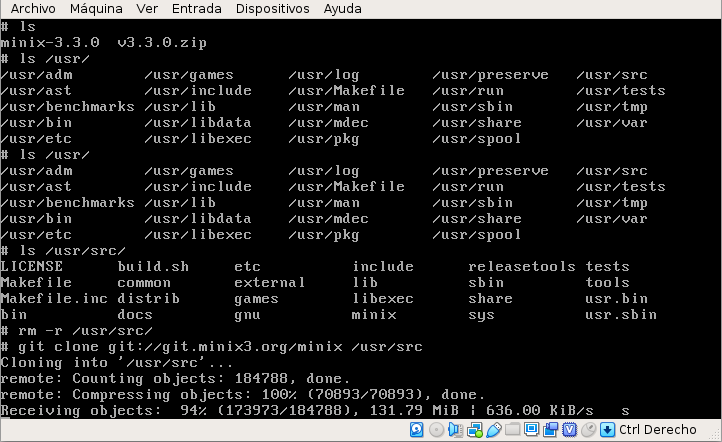
\includegraphics[width=0.7\textwidth]{0.png}
  \caption{Caption}
\end{figure}

\subsubsection{Cambio de rama de desarrollo}
\begin{figure}[H]
  \centering
  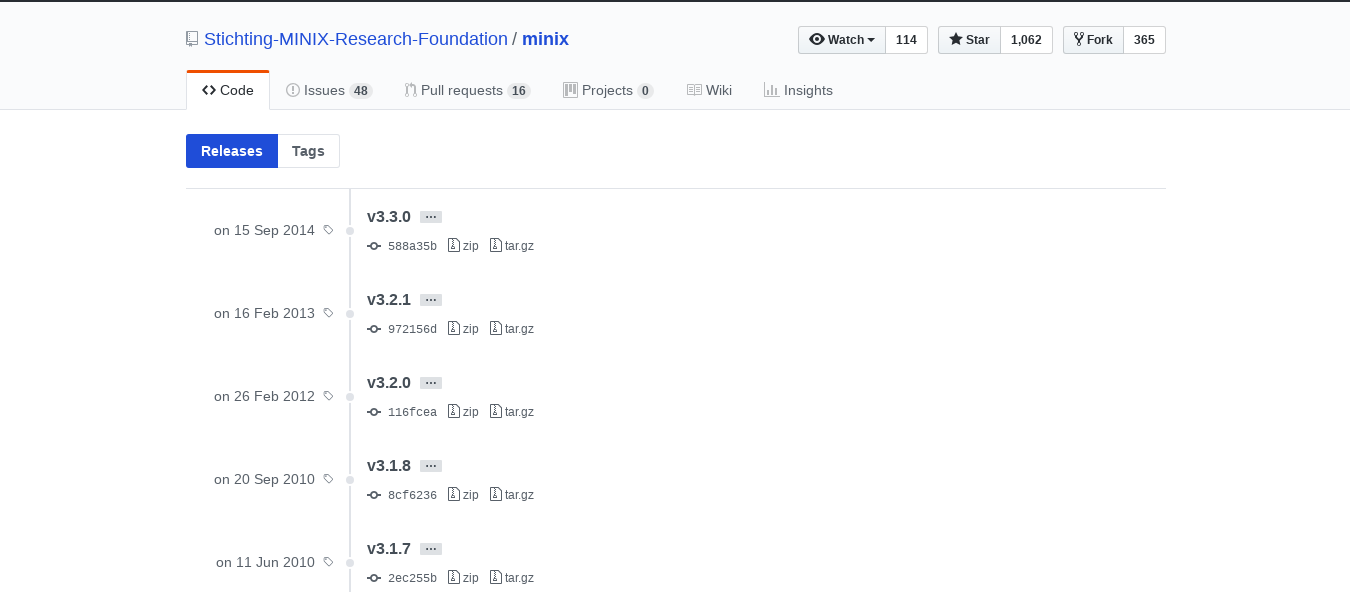
\includegraphics[width=0.7\textwidth]{1.png}
  \caption{Caption}
\end{figure}
\begin{figure}[H]
  \centering
  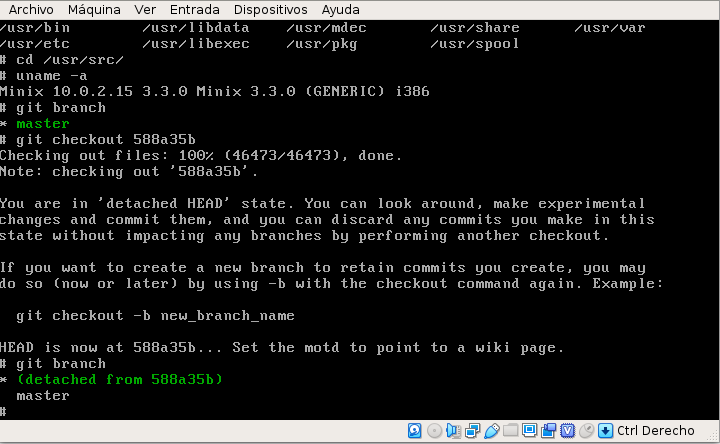
\includegraphics[width=0.7\textwidth]{2.png}
  \caption{Caption}
\end{figure}
\begin{figure}[H]
  \centering
  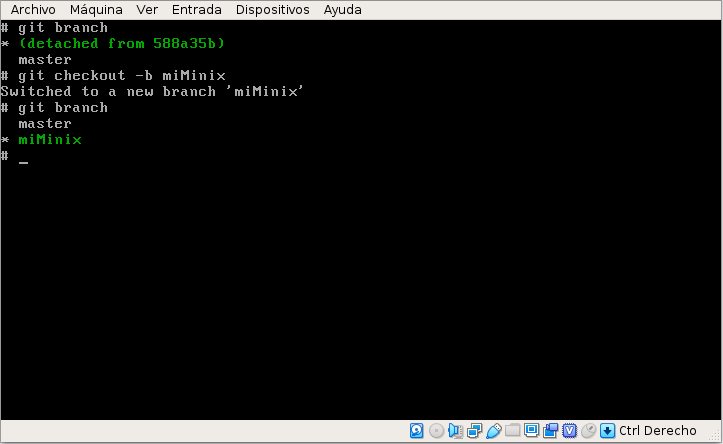
\includegraphics[width=0.7\textwidth]{3.png}
  \caption{Caption}
\end{figure}

\section{Modificación}

\subsection{Kernel}
\begin{figure}[H]
  \centering
  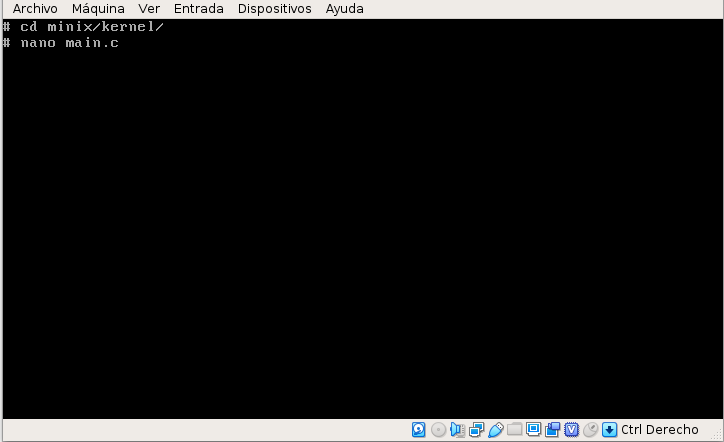
\includegraphics[width=0.7\textwidth]{4.png}
  \caption{Caption}
\end{figure}

\subsubsection{main.c}
\begin{figure}[H]
  \centering
  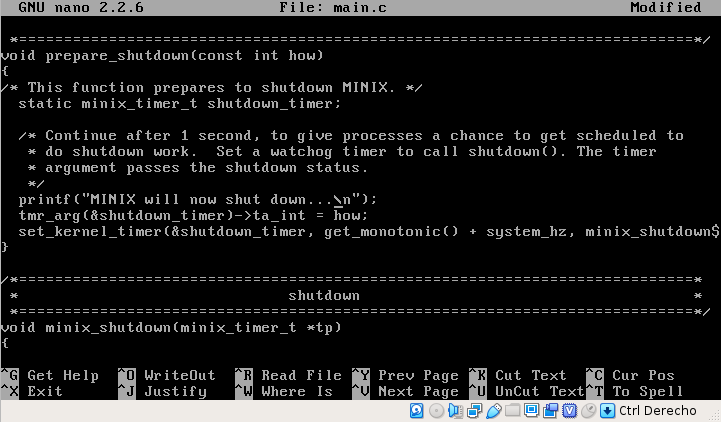
\includegraphics[width=0.7\textwidth]{5.png}
  \caption{Caption}
\end{figure}
\begin{figure}[H]
  \centering
  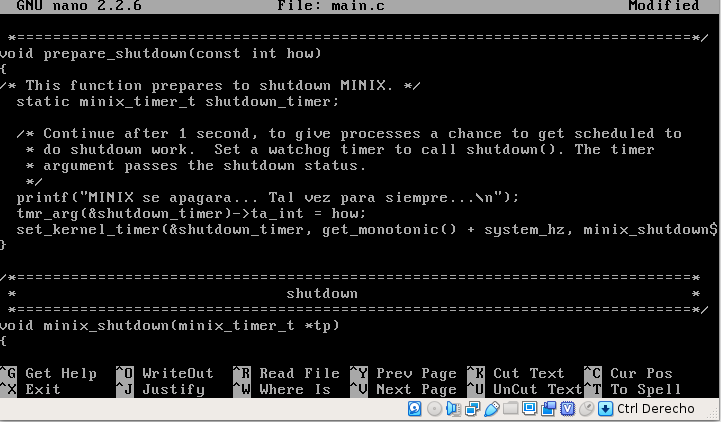
\includegraphics[width=0.7\textwidth]{6.png}
  \caption{Caption}
\end{figure}


\section{Recompilación}

\subsection{Creación de nueva imagen de arranque}
\subsubsection{Comando make}
\begin{figure}[H]
  \centering
  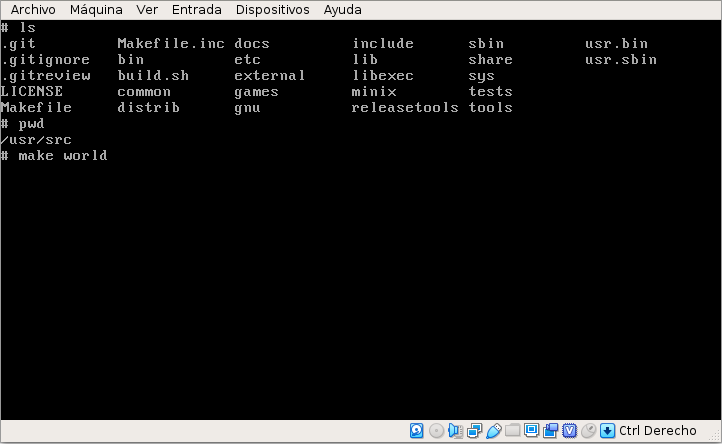
\includegraphics[width=0.7\textwidth]{7.png}
  \caption{Caption}
\end{figure}
\begin{figure}[H]
  \centering
  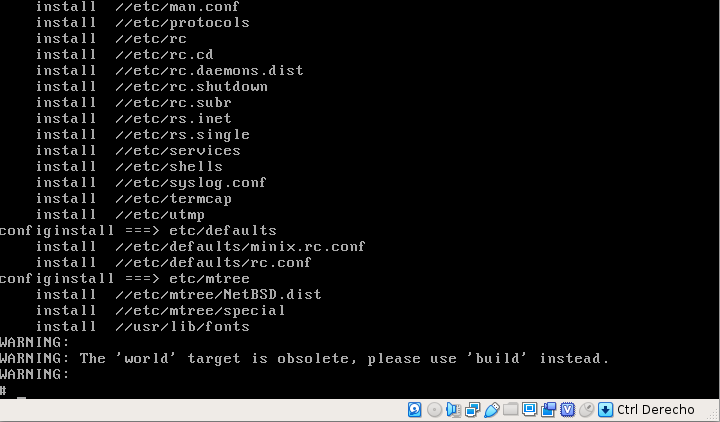
\includegraphics[width=0.7\textwidth]{8.png}
  \caption{Caption}
\end{figure}
\subsection{Verificación}
\subsection{Directorio /boot}
\begin{figure}[H]
  \centering
  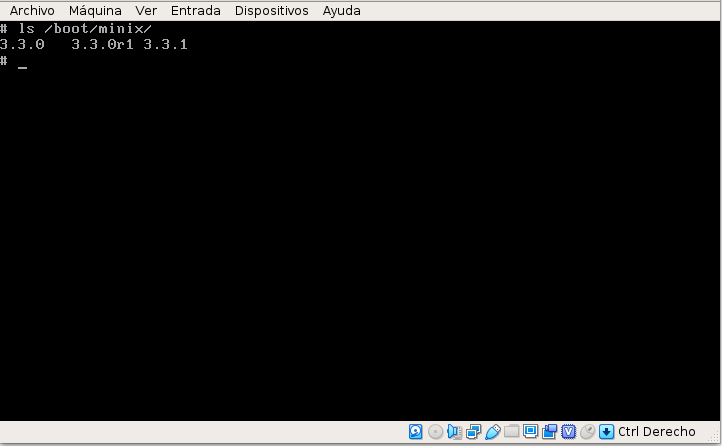
\includegraphics[width=0.7\textwidth]{12.png}
  \caption{Caption}
\end{figure}
\subsubsection{Reinicio}
\begin{figure}[H]
  \centering
  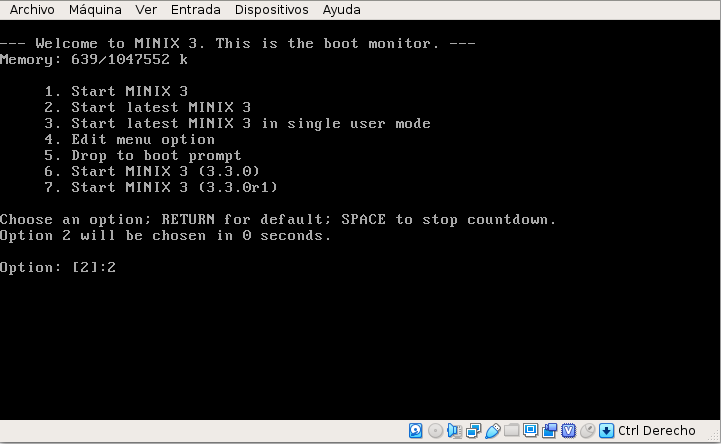
\includegraphics[width=0.7\textwidth]{9.png}
  \caption{Caption}
\end{figure}
\begin{figure}[H]
  \centering
  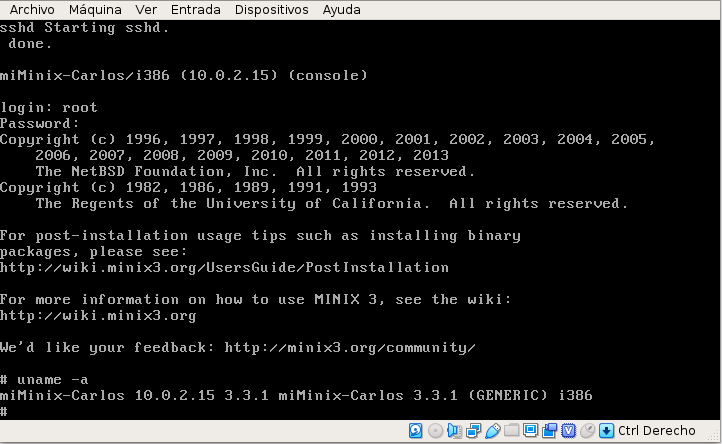
\includegraphics[width=0.7\textwidth]{10.png}
  \caption{Caption}
\end{figure}
\begin{figure}[H]
  \centering
  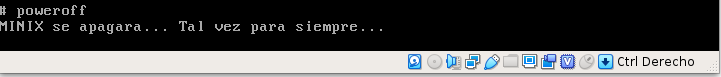
\includegraphics[width=0.7\textwidth]{11.png}
  \caption{Caption}
\end{figure}







\end{document}
